\documentclass[12pt,a4paper]{article}
\usepackage[latin1]{inputenc}
\usepackage{amsmath}
\usepackage{amsfonts}
\usepackage{amssymb}
\usepackage{graphicx}
\graphicspath{ {./images/} }
\usepackage{wrapfig}
\author{Zdenek Krousky}
\title{Easysleep}
\hyphenation{con-sti-tu-tion-al}

\renewcommand*\contentsname{Table of Content}

\begin{document}
	\begin{titlepage}
		\centering
		
\includegraphics[width=0.5\textwidth]{gmit_full1.png}\par\vspace{0cm}
		{\scshape\LARGE Galway - Mayo \par Institute of Technology \par}
		\vspace{1cm}
		{\scshape\Large Final year project\par}
		\vspace{1.5cm}
		{\Huge\bfseries Easysleep\par}
		\vspace{2cm}
		{\Large\itshape Zdenek Krousky\par}
		\vfill
		supervised by\par
		Paul \textsc{Lennon}
		
		\vfill
		
		% Bottom of the page
		{\large \today\par}
	\end{titlepage}
	
	\newpage
	\pagenumbering{gobble}
	\pagenumbering{arabic}
	\newpage
	
	\section*{Declaration}
	This project is presented in partial fulfilment of the requirements for the Degree of Bachelor of Engineering (Hons.) in Software and Electronic Engineering at Galway-Mayo Institute of Technology. This project is my own work, except where otherwise accredited. Where the work of others has been used or incorporated during this project, this is acknowledged and referenced.
	\newpage
	
	\section*{Acknowledgement}
	I would like to extend my thanks to my supervisor Paul Lennon who made sure I stay on track with my project as well as to Niall O'Keeffe for his support in embedded part of the project. I would also like to thank my wife Caroline for her ongoing support through my studies.
	\newpage
	\tableofcontents
	\newpage
	
	\section{Project background and motivation}
	{\bfseries Aim of the project, Why?}\\
	
	The goal of this project was to create a device that would help resolve nocturnal enurism (bedwetting) common in children above the age of 5. I am myself a parent of a child with  
	such difficulty and can relay to the stress this causes. Me and my wife have tried various  
	methods of resolving this such as encouriging my daughter going to the toilet prior to  
	going to the bed, waking her up during the night and medication.\\
	
	According to my research there is a number of different causes for this bedwetting to 
	happen. Medical reasons only account for close to 3%. 15% of children above the age of 
	5 still wet the bed at night and up to 5% above the age of 10 continue to do so. The selection 
	of night-time pants in grocery stores show sizes for children up to the age of 14.\\
	
	I have come to the conclusion, that the main cause of my child being wet every night is the 
	deep sleep. Her urge to go to the toilet simply isn't strong enough to wake her up at night.\\
	
	This is where my project comes in. It aims to resolve the nocturnal enurism of children 
	where the deep sleep is the root cause.
	\newpage
	
	\section{Overview}
	{\bfseries What is Easysleep?, Research, Architecture diagram}\\
	
	The project consists of two devices that are able to communicate via Bluetooth and a mobile phone application. The idea behindthe project is a master device capable of detecting moisture and recording the time and the data of this event. The master device can then notify the secondary one (bracelet) responsible for waking up the sleeping person on the following night prior to the event-time and also receive acknowledgement status. The master device can also communicate with a mobile phone application.  The user can silence an ongoing alarm, request current date and time of the system or change it and also request data of last ten events that would then be saved into an SQLite database on the phone for anytime access or for statistics/progress.
	\newpage
	
	\section{Hardware}
	{\bfseries Hardware used, Connections, Specifications}\\
	
	My project doesn't consist of to many parts. Aside from the actual microcontroller it only 
	requires a vibration motor, relay and buzzer all of which are used to wake the sleeping person  
	up. HC-05 bluetooth modules are used to facilitate communication between the master device and  
	the bracelet a mobile phone.
		\subsection{FRDM-K64F}
		\begin{figure}[h]
			\centering
			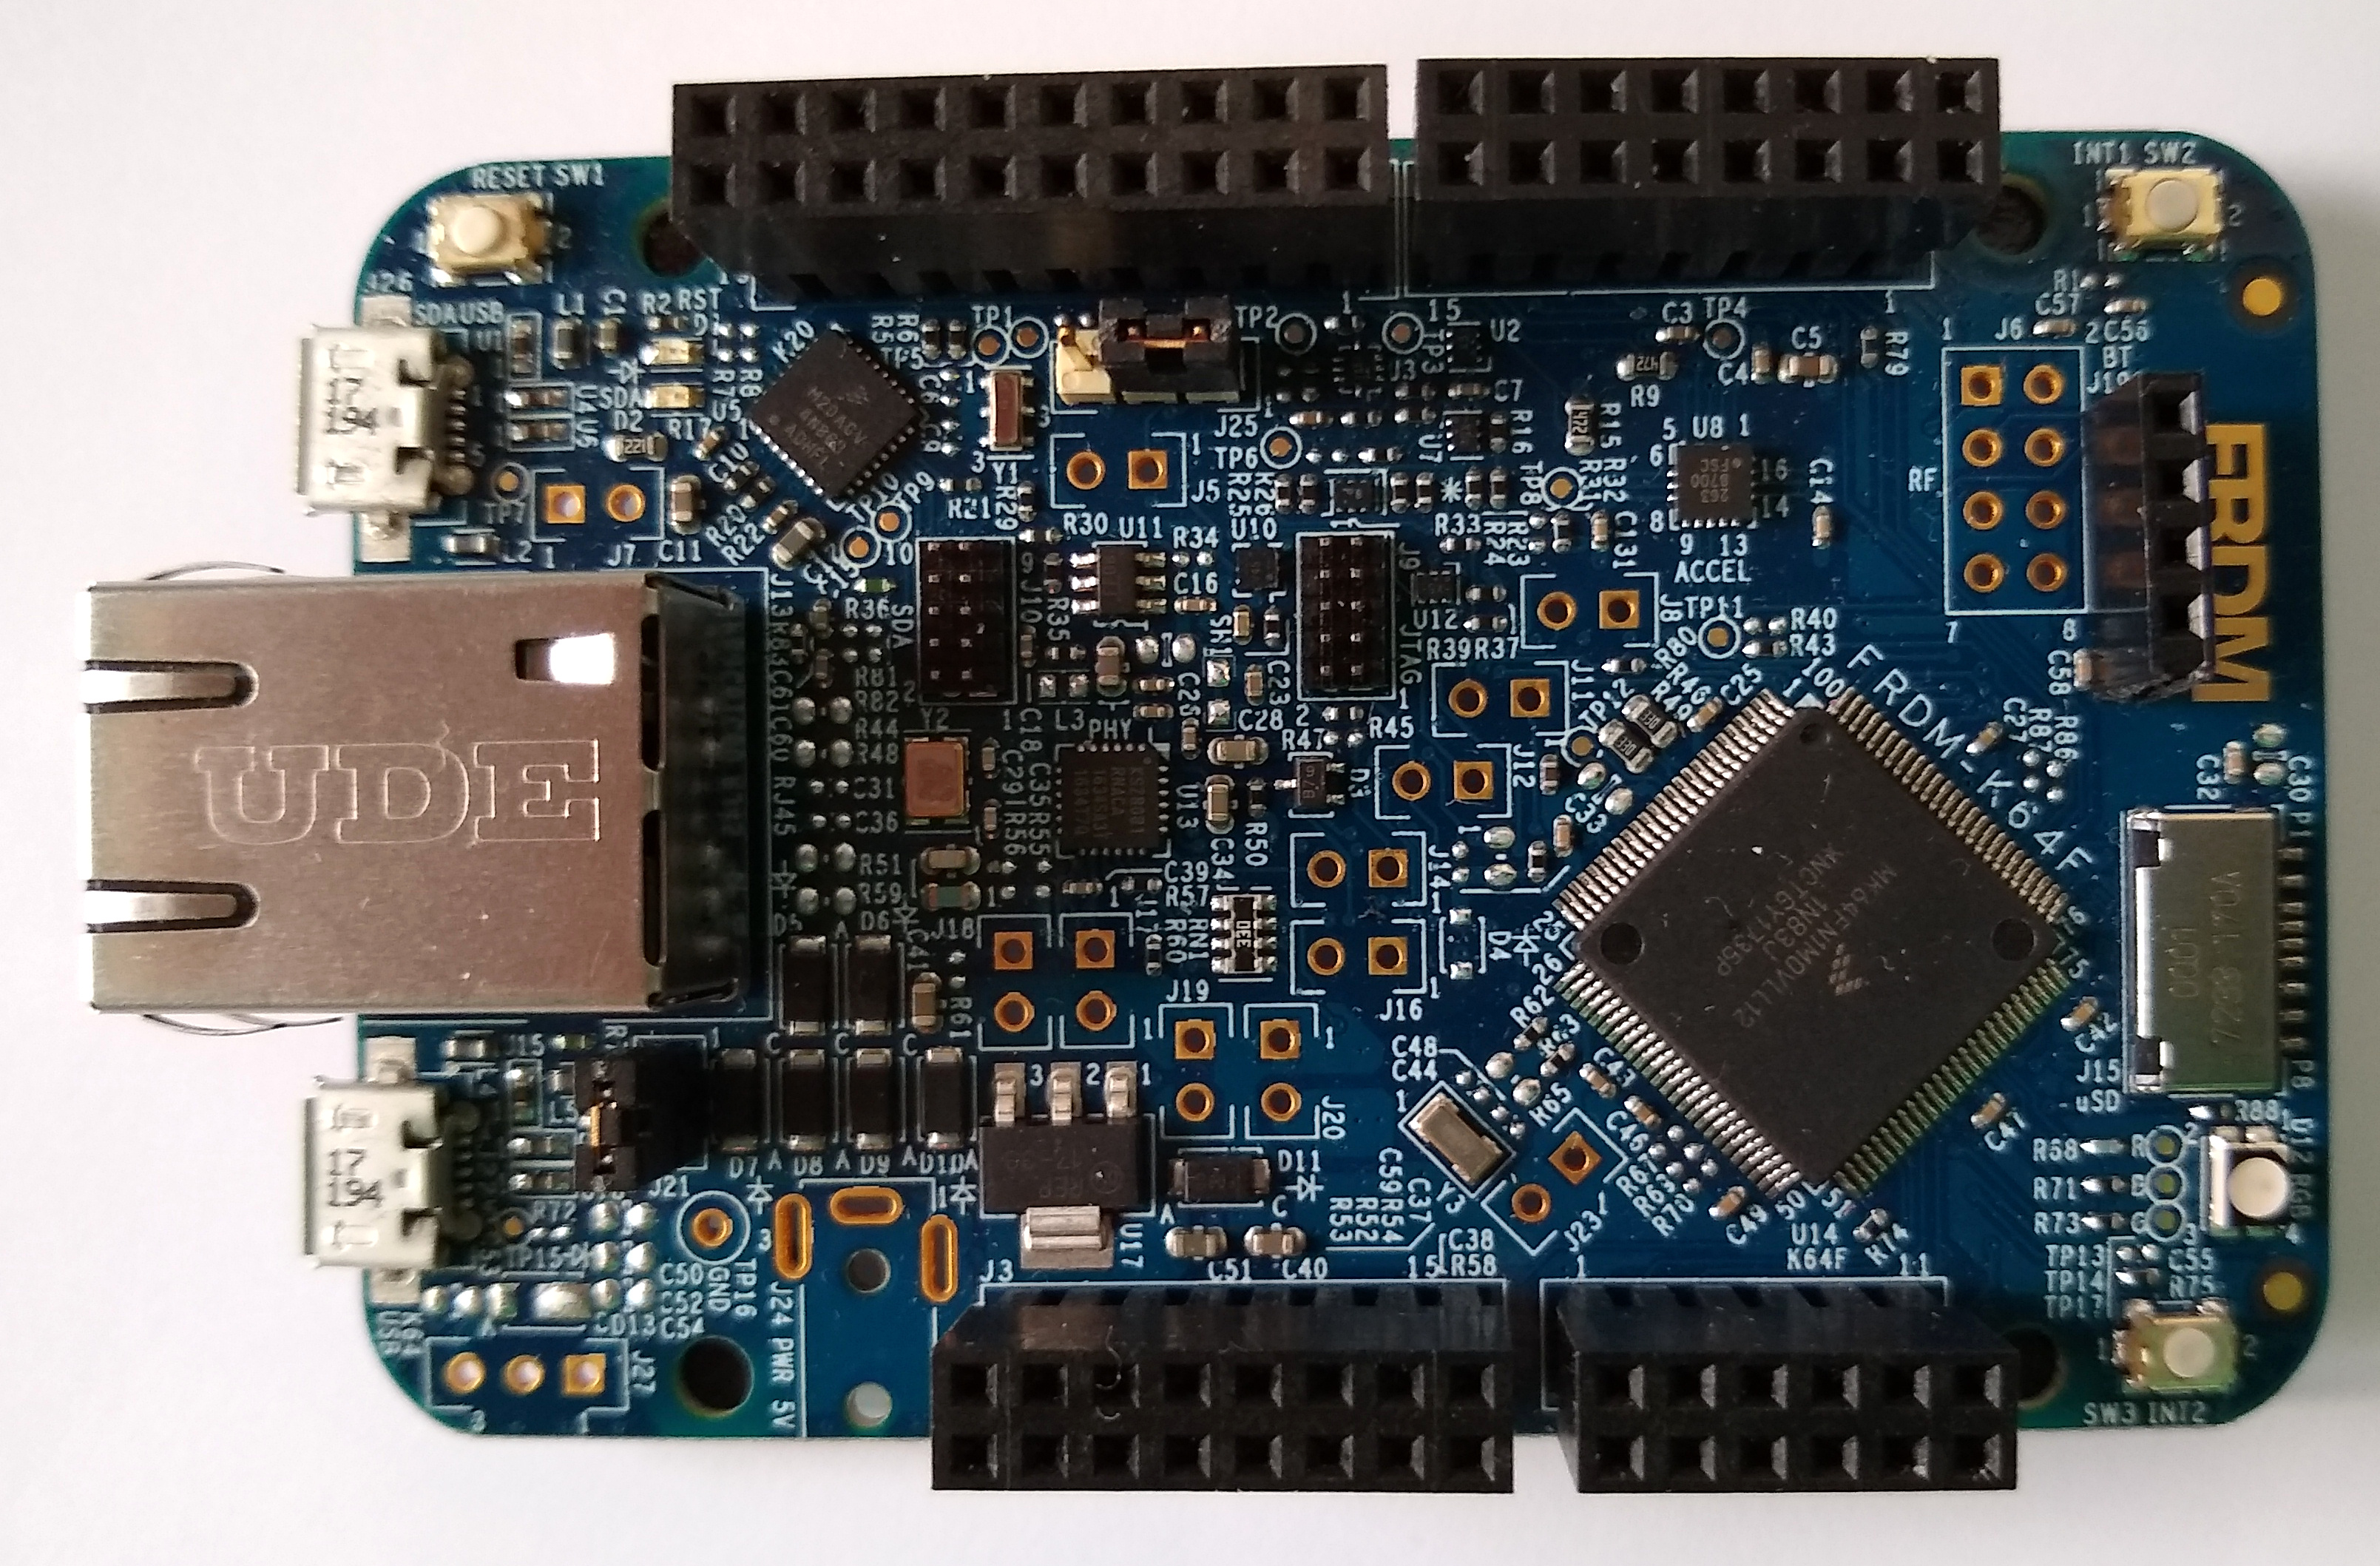
\includegraphics[width=0.7\textwidth]{k64f1.jpg}\par\vspace{0cm}
			\caption{FRDM-K64F development board}
		\end{figure}
		FRDM-K64F is a very capable development board manufactured by NXP Semiconductors with a 
		headquarters in Eindhoven, Netherlands and Austin, Texas. I have chosen this board because  
		of my familiarity with it and of its abilities. This board and its cousin KL25Z were used  
		throughout the course as part of the embedded systems modules.\\  	
		\\
		{\bfseries Board specifications:}  	
		\begin{itemize}
			\item 120MHz ARM Cortex-M4 microcontroller
			\item 1MB Flash memory
			\item 256kB RAM
			\item Ethernet
			\item SDHC
			\item low-power
			\item FXOS8700CQ accelerometer and magnetometer 
			\item Add-on Bluetooth module: JY-MCU BT board V1.05
			\item RGB LED
			\item 2x user push buttons
			\item form-factor compatible with Arduino Uno Rev.3 pin layout
		\end{itemize}
		
		\subsection{Parallax 28821 Vibration motor}	
		\begin{wrapfigure}{r}{0.25\textwidth}
			\centering
			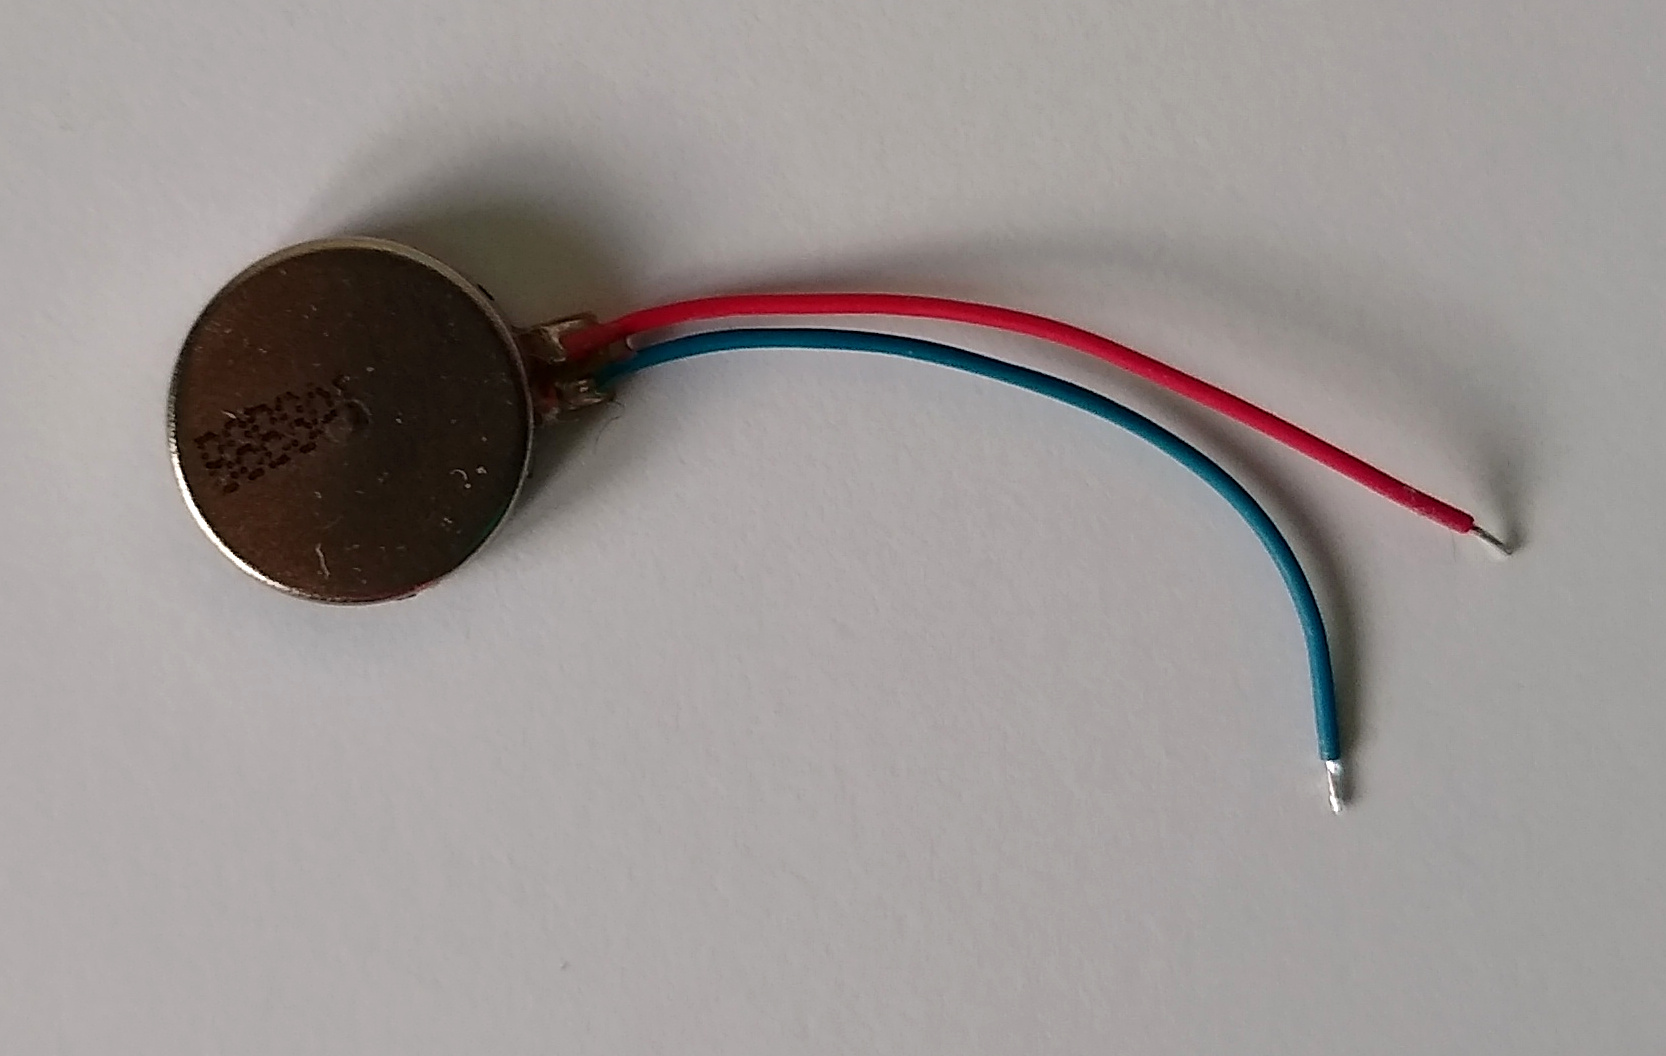
\includegraphics[width=0.2\textwidth]{parallax_vib_mot1.jpg}
			\caption{Parallax vibration motor}
		\end{wrapfigure}
		
		The vibration motor is used to gently and quietly wake the sleeping person up in the first stage of the overall wake-up process. Parallax vibration motor seemed appropriate device for this task as it requires only 3V of power. However, the current it requires is quite high and cannot be supplied by the K64F thus an external supply has to be used.\\
		
		\begin{figure}[h]
			\centering
			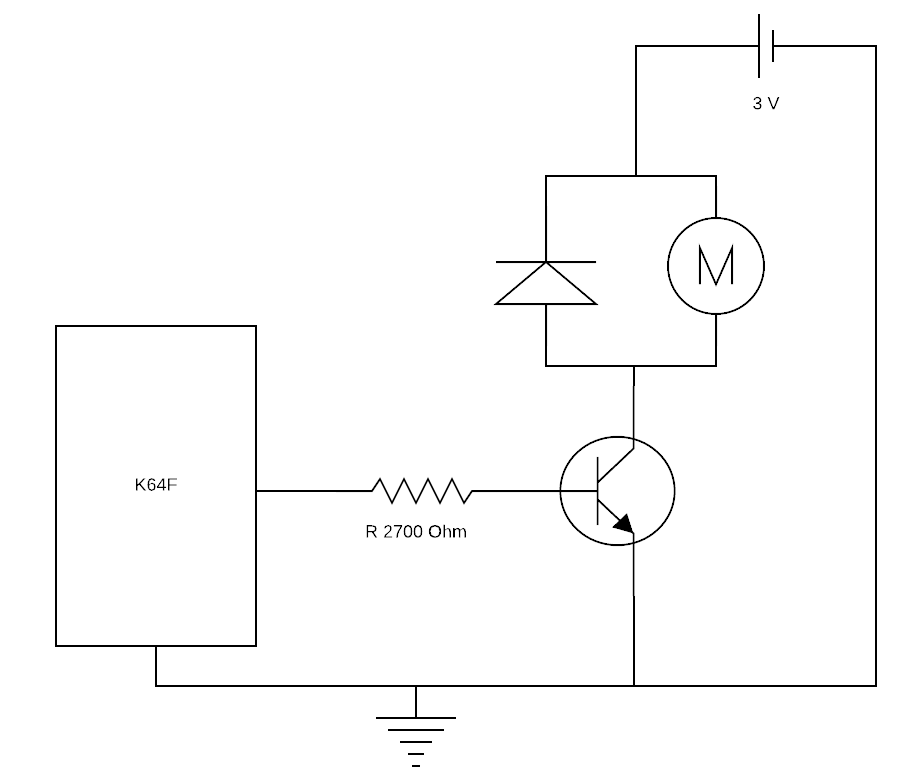
\includegraphics[scale=0.3]{motor_diag1.png}
			\caption{Vibration motor connection diagram}
		\end{figure}

		{\bfseries Motor specifications:}
		\begin{itemize}
			\item Rate voltage: 3.0V
			\item Rate current: 150mA
			\item Rate speed: 9,000r/min Min
			\item Starting voltage: 2.3V
		\end{itemize}

		\subsection{Buzzer}
		The buzzer is used for third stage of wake-up process if the vibration motor or relay fail 
		to wake the sleeping person. This is a passive device and for the sound to be produced  
		the Flex Timer Module of K64F is used to generate PWM signal on the connected GPIO pin.
		
		\subsection{HC-05 Bluetooth module}
		
		\begin{wrapfigure}{l}{0.25\textwidth}
			\centering
			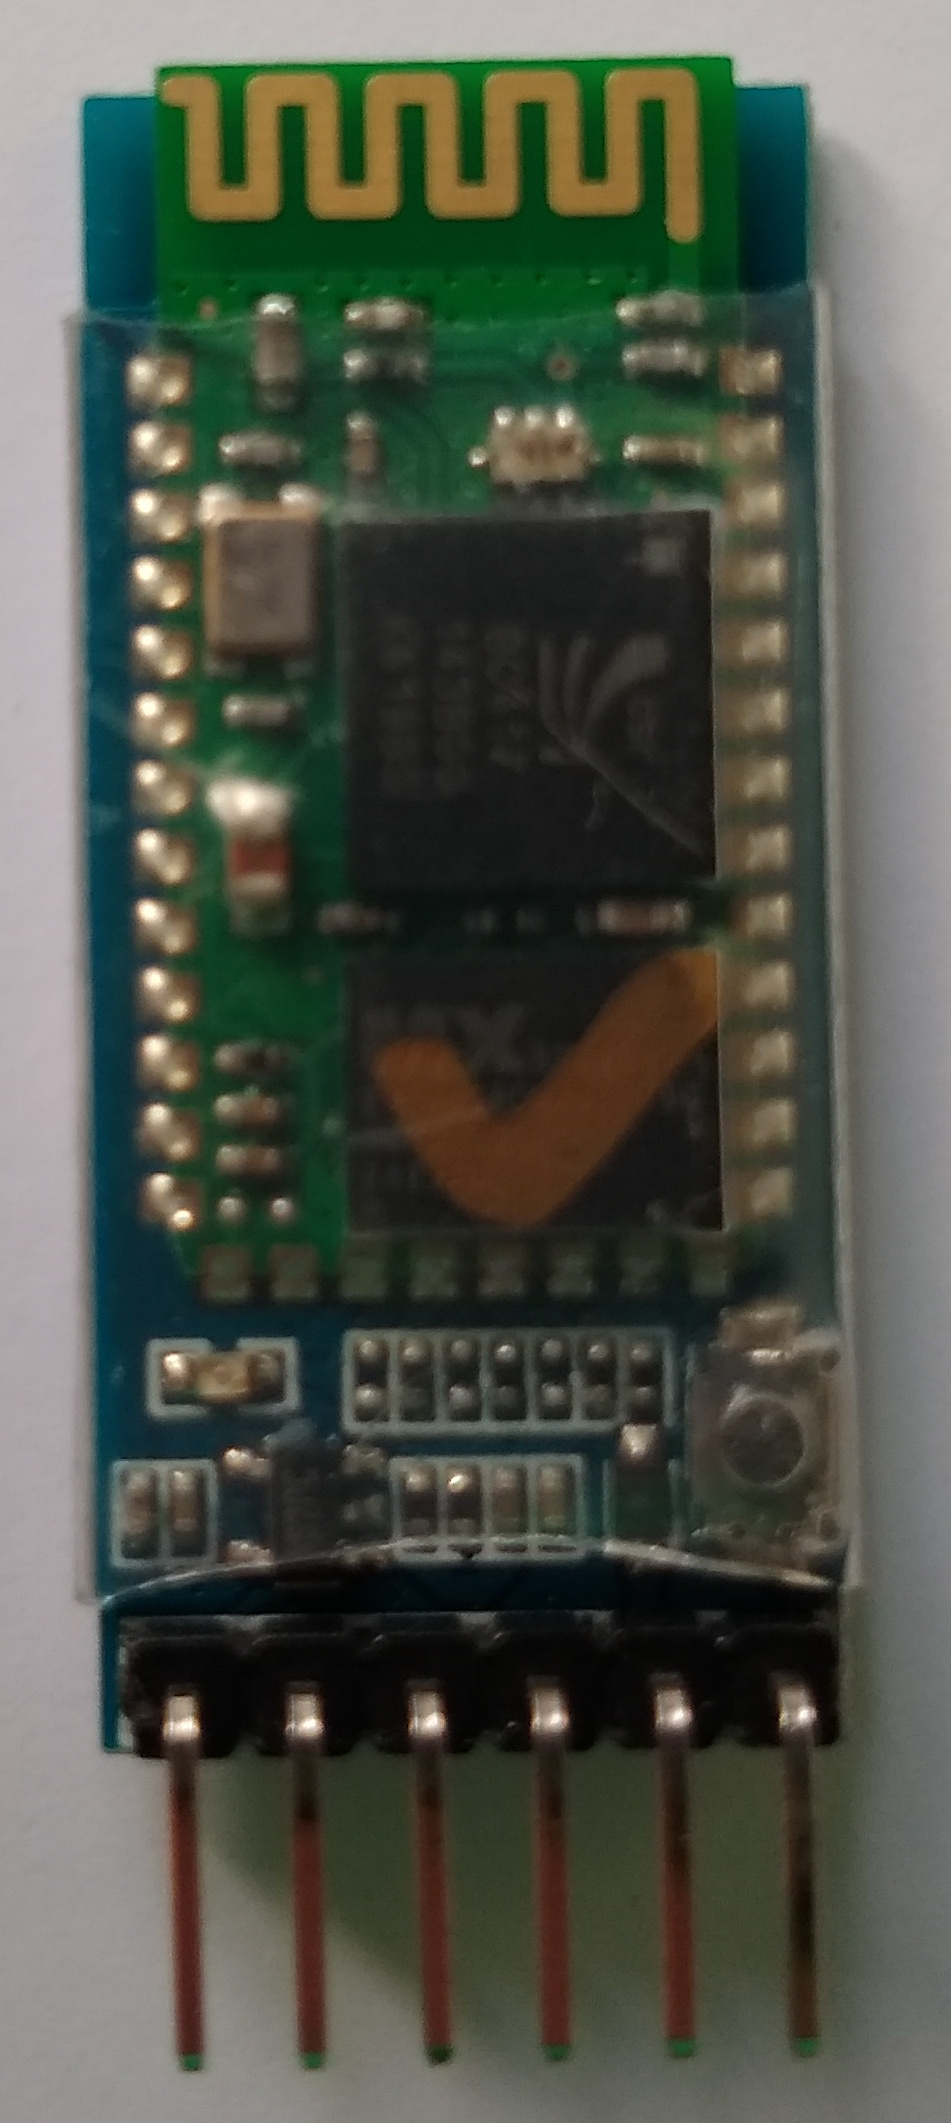
\includegraphics[scale=0.06]{hc-05_1.jpg}
			\caption[HC-05 Bluetooth module]{HC-05}
		\end{wrapfigure}

		HC-05 is commonly used Bluetooth module often used with Arduino projects. The K64F supports  
		this module also. I have installed small section of header pins to house this module. For my  
		project I am using two of these. One to communicate with the secondary device (bracelet) and  
		second one to communicate with the mobile phone.\\
		
		This module can operate as a master or as a slave. Unfortunately it only supports one-to-one  
		communication and that was the reason for adding the second module.\\\\\\
		
		{\bfseries Configuration:}
		\begin{itemize}
			\item Baudrate: 38400
			\item 8 bit length
			\item 1 stop bit
			\item no parity

		\end{itemize}
		\newpage
		
	\section{Software}
	{\bfseries Software used, Programming languages, IDEs, Software tools}\\
	Througout my project I have used various software tools to develop C and Java code, as well as
	software to monitor the behaviour of the system.
	
		\subsection{MCUXpresso}
		I have used MCUXpresso 11.1 to develop code for K64F. This is an Eclipse based IDE tailored to suit NXP devices. There are lots of alternatives for other manufacturers such as Atollic Studio for STM32. I have became familiar with this IDE through my time in the college as it 
		was used for code development in embedded systems classes. I have also used this IDE during my work placement in Jaguar LandRover.\\
		
		The project uses Amazon FreeRTOS to efficiently manage various tasks of the system. This is an open-source real-time operating system and it's usage greatly reduces the complexity of  C code used for functionality of the system. A programmer can divide the code into smaller, easier to manage blocks known as tasks. A communication between those is facilitated by usage of semaphores, notifications and queues.\\
		
		Prior to commencement of work on the project I had to obtain appropriate Software
		Development Kit. I did so, through SDK Builder present on NXP website. This site allowed 
		me to select specific processor and middleware and generated an SDK package that I then 
		imported into the MCUXpresso. This package included all necessary drivers for various 
		peripherals present on the development board such as GPIO or FlexTimer driver.\\
		
		I also had to create a repository on Github to have a proven record of my work required 
		by my supervisor and other lecturers and also to have a safety net in case things go 
		wrong. This is an amazing tool to know and use. I was grateful to have the ability of 
		reverting to previous revisions of my code throughout the development as few times the  
		path I have chosen to steer the development proved unsuitable and it would have been  
		impossible to revert changes from memory.\\
		    
		\newpage
	
		\subsection{Android Studio}
		mobile application development
		\newpage
		
		\subsection{Other}
		SystemView, FreeRTOS, Pulseview, Git/Github, project management software, BT configuration,
		Doxygen
		\newpage
	
	\section{Conclusion}
	what was the development of the project like
	\newpage
	
	\section{References}
	\newpage
	
	\section{Bibliography}
	\newpage
	
	\listoffigures
	
\end{document}